\documentclass[12pt]{article}
 \usepackage[margin=1in]{geometry} 
\usepackage{amsmath,amsthm,amssymb,amsfonts, pgfplots}
\usepackage{stackengine}
 
 \newcommand{\longdiv}[2]{$#1\overline{\smash{)}#2}$}
\newcommand{\N}{\mathbb{N}}
\newcommand{\Z}{\mathbb{Z}}
 
\newenvironment{problem}[2][Problem]{\begin{trivlist}
\item[\hskip \labelsep {\bfseries #1}\hskip \labelsep {\bfseries #2.}]}{\end{trivlist}}
 
\begin{document}
\title{Pg. 120-121, #1-6, 8, 1, 12-14, 16}
\date{October 13, 2018}
\author{Mia Jones}

\maketitle

\begin{problem}{1}
In a line graph, points that represent data pairs are plotted using the scales on the \boxed{\text{x axis}} and \boxed{\text{y axis.}}
\end{problem}

\begin{problem}{2}
Bar graphs compare numbers from data sets, whereas line graphs are used for showing data over time.
\end{problem}

\begin{problem}{3}
\boxed{\text{21 bottled drinks.}}
\end{problem}

\begin{problem}{4}
\boxed{\text{24 cartons.}}
\end{problem}

\begin{problem}{5}
\boxed{\text{Canned drinks.}}
\end{problem}

\begin{problem}{6}
\boxed{\text{Bottled drinks.}}
\end{problem}


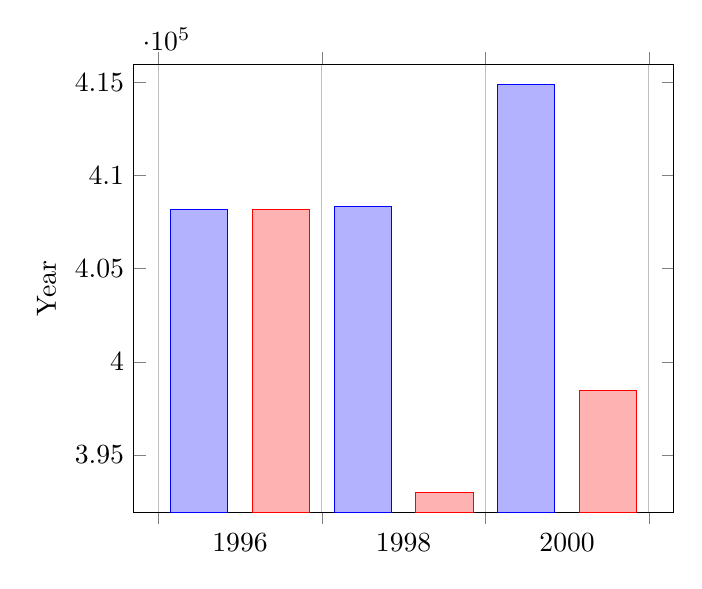
\begin{tikzpicture}
\begin{axis}[
	x tick label style={
		/pgf/number format/1000 sep=},
	ylabel=Year,
	enlargelimits=0.05,
	ybar interval=0.7,
]
\addplot 
	coordinates {(1996,408184) (1998,408348)
		 (2000,414870) (2002,412156)};
\addplot 
	coordinates {(1996,408192) (1998,393007) 
		(2000,398449) (2002,395972)};
\end{axis}
\end{tikzpicture}

\end{document}